% Use custom color mediblue CMYK 1,0,0,0.3 for all blue elements. In RGB it is around 0,50,70 (0..100) or 0,126,178 (0..255).
\documentclass[portrait,final,a0paper,fontscale=0.320]{imiseposter}
\usepackage[T1]{fontenc}
\usepackage[utf8]{inputenc}
\usepackage[ngerman]{babel}% change to ngerman for a German poster
\microtypecontext{spacing=nonfrench}
% Using biblatex and biber. It's more modern but takes more than twice as long to compile in my case. ****
% If you use biblatex, you need to comment and uncomment the marked statements in the references as well.
\usepackage{csquotes}
%\usepackage[style=numeric,backend=biber]{biblatex}
%\addbibresource{poster.bib}
%*********************************************************************************************************
\usepackage{graphicx}
\usepackage{url}% do not use hyperref as its links are displaced with baposter because of the font scale 
\usepackage{booktabs}
\usepackage{caption}

% Select Font %%%%%%%%%%%%%%%%%%%%%%%%%%%%%%%%%%%%%%%
%\usepackage{helvet} % closest to arial
\usepackage{bookman} % has some resemblance to Futura
%%%%%%%%%%%%%%%%%%%%%%%%%%%%%%%%%%%%%%%%%%%%%%%%%%%%%
\renewcommand{\familydefault}{\sfdefault}

%\newcommand{\captionfont}{\footnotesize}
\usepackage[font=small,labelfont=bf]{caption}

\newcommand{\imagebox}[3]{
\begin{minipage}{\linewidth}
\centering
\captionof{figure}{#1}
\includegraphics[width=#2\textwidth]{#3}
\end{minipage}
}

\usepackage{tcolorbox}
\newtcolorbox{subsectionbox}[1]
{
  colframe=white,
  colback=white,
  colbacktitle=mediblue,
  sharp corners=all,
  title    = {#1},
}
\begin{document}

\begin{poster}% Set grid to false for final print
  {grid=false,}
  % Eye Catcher
  {}
  % Title
  {Anthropological Notation Ontology}
  % Authors
  {Konrad Höffner, Andy Ludwig, Marie Heuschkel\\Marleen Mohaupt, Dirk Labudde, Alexandr Uciteli}
  %{Alexandr Uciteli, Konrad Höffner{\small <konrad.hoeffner@imise.uni-leipzig.de>}, Andy Ludwig, other Author, Another Author}
  % University logo
  {% The makebox allows the title to flow into the logo, this is a hack because of the L shaped logo.
    %\includegraphics[height=9.0em]{img/medfak.pdf}
  }

%%%%%%%%%%%%%%%%%%%%%%%%%%%%%%%%%%%%%%%%%%%%%%%%%%%%%%%%%%%%%%%%%%%%%%%%%%%%%%
\begin{posterbox}[name=background,column=0,row=0]{Hintergrund}
%Ziel des SaxFDM-Projektes ist die Entwicklung einer Ontologie für die einheitliche Einordnung von Knochenfunden aus Ausgrabungen in das Skelettsystem, die Beschreibung der Skelettstücke sowie die Definition von Funktionen zur Ableitung verschiedener Phänotypen des Menschen. 
Daten aus der historischen und forensischen Anthropologie und der modernen Rechtsmedizin erlauben ein Verständnis über das Verhalten, die Lebensweise und Kultur des Menschen aus verschiedenen Zeitepochen.
Somit sind Daten von Ausgrabungen, in denen menschliche Überreste sowie Kulturgüter, ehemalige Behausungen usw. zutage gefördert und untersucht werden, die Grundlage für zukünftige Analysen.

\end{posterbox}
%%%%%%%%%%%%%%%%%%%%%%%%%%%%%%%%%%%%%%%%%%%%%%%%%%%%%%%%%%%%%%%%%%%%%%%%%%%%%%
\begin{posterbox}[name=methods,below=background]{Methoden}
Um Information aus Knochenfunden abzuleiten, wird in der Anthropologie auf die Osteometrie zurückgegriffen.
Die Osteometrie beschreibt die Vermessung des Skeletts.
Dabei wird quantitativ Größe und Form von Skelettelementen eines Individuums erfasst.
Grundlage dafür sind vorab definierte Punkte, die osteometrischen Landmarken, die auf den zu vermessenden Skelettelementen markiert sind~\cite{forensicanthropology}.
Die Messstrecken zwischen diesen Landmarken werden mittels eines standardisierten Verfahrens mit bestimmten Messwerkzeugen abgenommen.

~\\\imagebox{Prozess der Rekonstruktion vergangener Leben.~\cite{spurenlesen}}{1}{img/rekonstruktion.jpg}
Bei der osteometrischen Untersuchung entstehen Probleme:
Skelettelemente können nur ortsgebunden untersucht werden, was einen Transport über weite Strecken notwendig macht.
Dabei treten sowohl durch den Transport als auch während der Vermessung Abnutzungserscheinungen auf.
Dies ist besonders bei alten und porösen Funden problematisch und kann zu Abweichungen der Befunde führen.~\cite{praehistorischeanthropologie}

Ein digitaler Zwillings vermeidet diese Probleme.
Dabei wird das Element in einer virtuellen Untersuchungsumgebung dreidimensional modelliert; der Fund kann ortsungebunden und zeitgleich von mehreren Forschenden analysiert werden.
Trotz einer Beisetzung des Originals bleibt der Fund für die Nachwelt zugänglich.~\cite{digitalisierung}

Zur Erstellung der 3D-Modelle von menschlichen Knochen für die anthropologische Untersuchung und Annotation wird die Fotogrammmetrie eingesetzt.
Fotogrammmetrie beschreibt die Vermessung von Objekten in Fotografien.
Dabei können Entfernungen und Flächen bestimmt sowie geometrische Daten berechnet und Karten erstellt werden.
Für die dreidimensionale Analyse wird eine stereoskopische Betrachtung genutzt.
Dreidimensionale Koordinaten sind einfach berechenbar, wenn von einem Objekt zwei oder mehr Fotografien aus unterschiedlichen Perspektiven aufgenommen wurden.~\cite{digitalphotogrammetry}
\end{posterbox}
%%%%%%%%%%%%%%%%%%%%%%%%%%%%%%%%%%%%%%%%%%%%%%%%%%%%%%%%%%%%%%%%%%%%%%%%%%%%%%
\begin{posterbox}[name=results,column=1]{Ontologie}
Die Vereinheitlichung der Analyse von Knochenfunden erfolgt durch eine Ontologie.
Existierende Anatomie-Ontologien unterscheiden sich in der medizinischen und anthropologischen Sicht und berücksichtigen Aspekte wie den Abnutzungsgrad der Knochen nicht.\\
~\\\imagebox{Die Module der ANNO-Ontologie.}{1}{img/anno.pdf}
\iffalse
\begin{tabular}{ll}
\toprule
\textbf{Modul}			&\textbf{Inhalt}\\
\midrule
bones					&Knochen\\
dentes					&Zähne\\
anatomical locations	&Lage- und Richtungsbezeichnungen\\
osteological terms		&Begriffe zur Beschreibung des Skelettsystems\\
osteometric landmarks	&vordefinierte Punkte auf Skelettelementen\\
anatomical landmarks	&anatomische Punkte und Strukturen\\
\bottomrule
\end{tabular}
\fi
%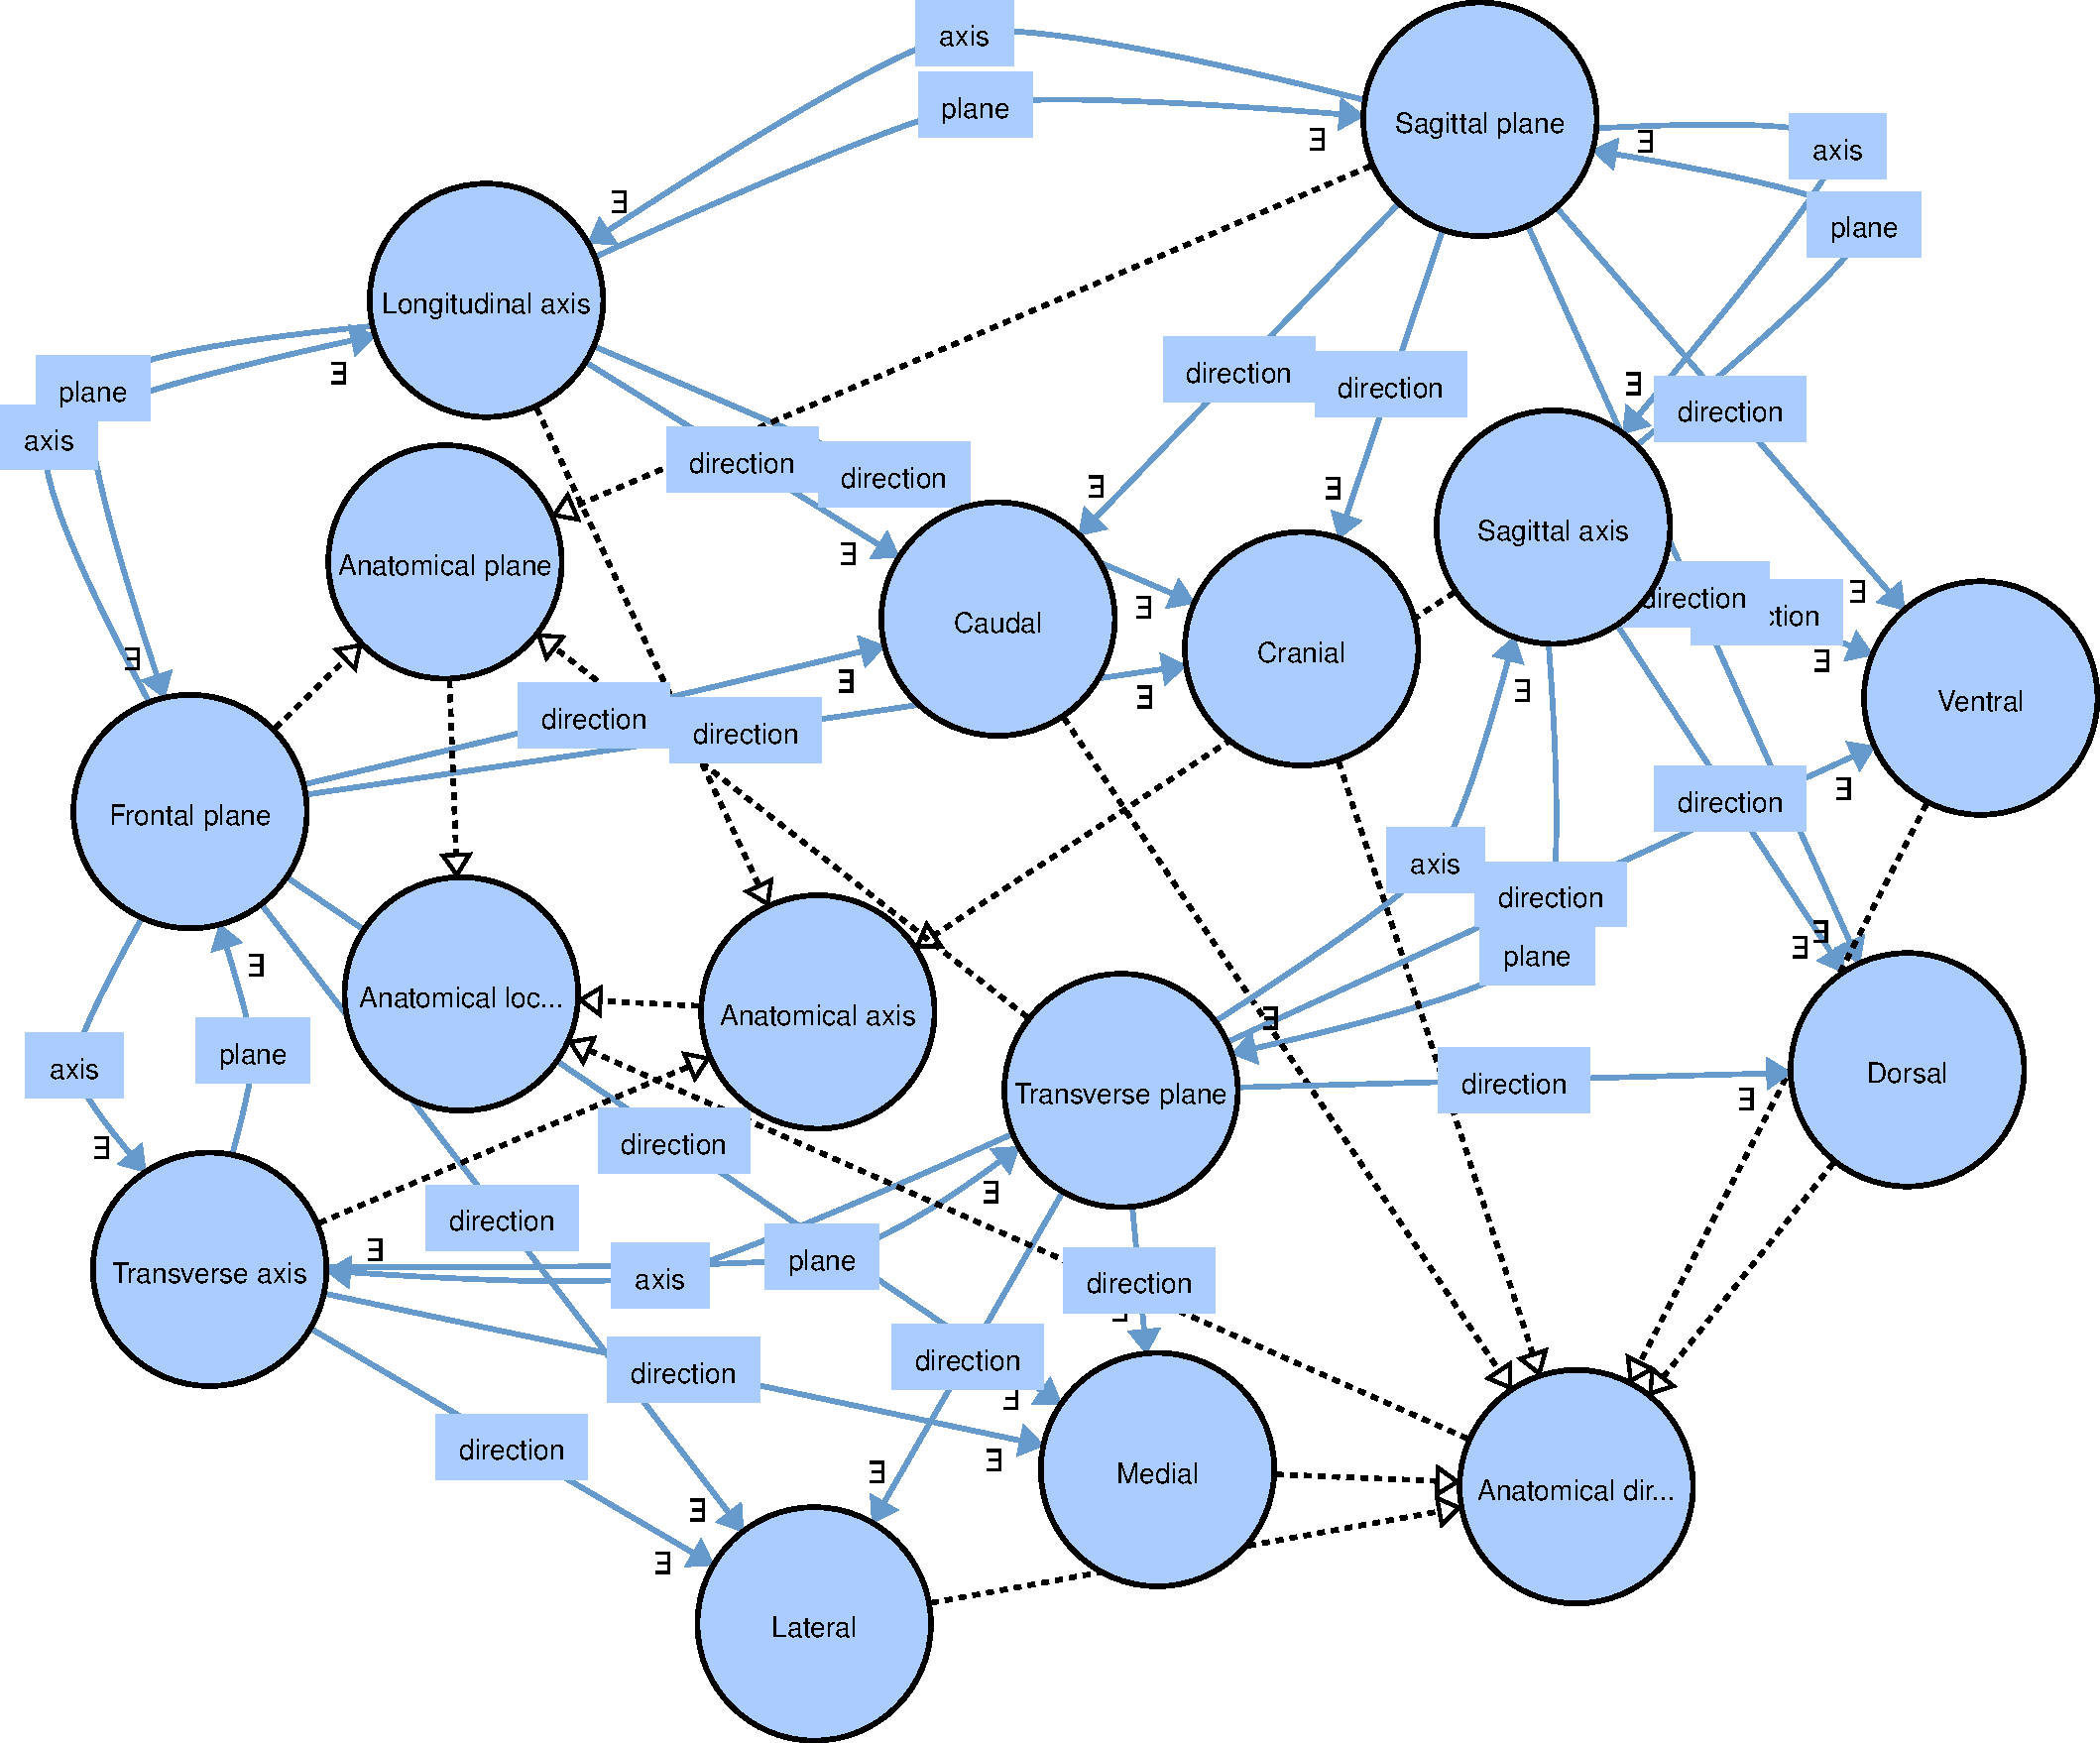
\includegraphics[width=0.8\textwidth]{img/location.pdf}
\imagebox{Lage- und Richtungsbezeichnungen der \emph{anatomical locations}.}{0.8}{img/location.pdf}
%\begin{subsectionbox}{OLS~\cite{ols}~\small\url{https://ols.imise.uni-leipzig.de/ontologies/anno}}
\iffalse
\begin{itemize}
\item Visualisierungen der Beziehungen zwischen Klassen
\item Synchronisation mit NFDI über API
\item Download in Semantic-Web-Standardformaten
\end{itemize}
\fi
%\imagebox{OLS~\cite{ols}~\small\url{https://ols.imise.uni-leipzig.de/ontologies/anno}}{1}{img/ols.png}
\imagebox{Die Ontologie wird durch den Terminologieserver \texttt{https://ols.imise.uni-leipzig.de/ontologies/anno} bereitgestellt.}{1}{img/ols.png}
%\end{subsectionbox}



\end{posterbox}
%%%%%%%%%%%%%%%%%%%%%%%%%%%%%%%%%%%%%%%%%%%%%%%%%%%%%%%%%%%%%%%%%%%%%%%%%%%%%%
%\begin{posterbox}[name=discussion,column=1,below=results]{Discussion}
%\end{posterbox}
%%%%%%%%%%%%%%%%%%%%%%%%%%%%%%%%%%%%%%%%%%%%%%%%%%%%%%%%%%%%%%%%%%%%%%%%%%%%%%
\begin{posterbox}[name=references,column=0,below=methods]{Literaturangaben}
    \small
\begingroup
    \renewcommand{\section}[2]{}%suppress heading
    % using bibtex ***********
    \bibliographystyle{abbrvdin}
    \bibliography{anno}
    % using biblatex *********
    %\printbibliography
    %*************************
    \endgroup
    \vspace{0.3em}
\begin{tabular}{p{33em}l}
\vspace{-3em}Diese Maßnahme wird mitfinanziert mit Steuermitteln auf Grundlage des vom Sächsischen Landtag beschlossenen Haushaltes.	&\vspace{-1em}
\includegraphics[height=0.03\textheight]{img/sachsen-signet.pdf}\\
\end{tabular}
\end{posterbox}
%%%%%%%%%%%%%%% Anno Logo
 \node [anchor=south east, inner sep=1pt,xshift=14em,yshift=-14em] at (current page.north west)
 {
\includegraphics[height=0.105\textheight]{img/anno-logo-short-mediblue.pdf}};
%%%%%%%%%%%%%%%  Founded by SaxFDM, their guidelines say to use the Saxony signet
 %\node [anchor=south east, inner sep=1pt,xshift=-3.5em] at (current page.south east) % for unknown reasons the xshift is necessary
 \node [anchor=south east, inner sep=1pt,xshift=-8.5em,yshift=-13em] at (current page.north east) % for unknown reasons the xshift is necessary
 %{\includegraphics[height=0.03\textheight]{img/dfg-logo.pdf}
 {
\includegraphics[height=0.08\textheight]{img/sachsen-signet.pdf}};
%%%%%%%%%%%%%%% Medical Faculty Logo
 \node [anchor=south east, inner sep=1pt,xshift=-17em,yshift=-2em] at (current page.south east)
 {\includegraphics[height=4cm,decodearray=0 0 0 0 0 1]{img/medfak.pdf}};
%%%%%%%%%%%%%%% Hochschule Mittweida
 \node [anchor=south east, inner sep=1pt,xshift=-19em,yshift=8em] at (current page.south east)
 {
\includegraphics[height=2.2cm]{img/mittweida-logo-mediblue.pdf}};
%%%%%%%%%%%%%%% FoSIL
 \node [anchor=south east, inner sep=1pt,xshift=-3.5em,yshift=7.9em] at (current page.south east)
 {
\includegraphics[height=2.2cm]{img/fosil-logo.png}};
%%%%%%%%%%%%%%% IMISE Logo
 \node [anchor=south east, inner sep=1pt,xshift=-3em,yshift=2em] at (current page.south east)
 {
\includegraphics[height=1.5cm]{img/imise-logo.pdf}};
%%%%%%%%%%%%%%%%%%%%%%%%%%%%%%%%%%%%%%%%%%%%%%%%%%%%%%%%%%%%%%%%%%%%%%%%%%%%%%
\end{poster}
\end{document}
